\section{Modelo clásico}

\begin{figure}[t!]
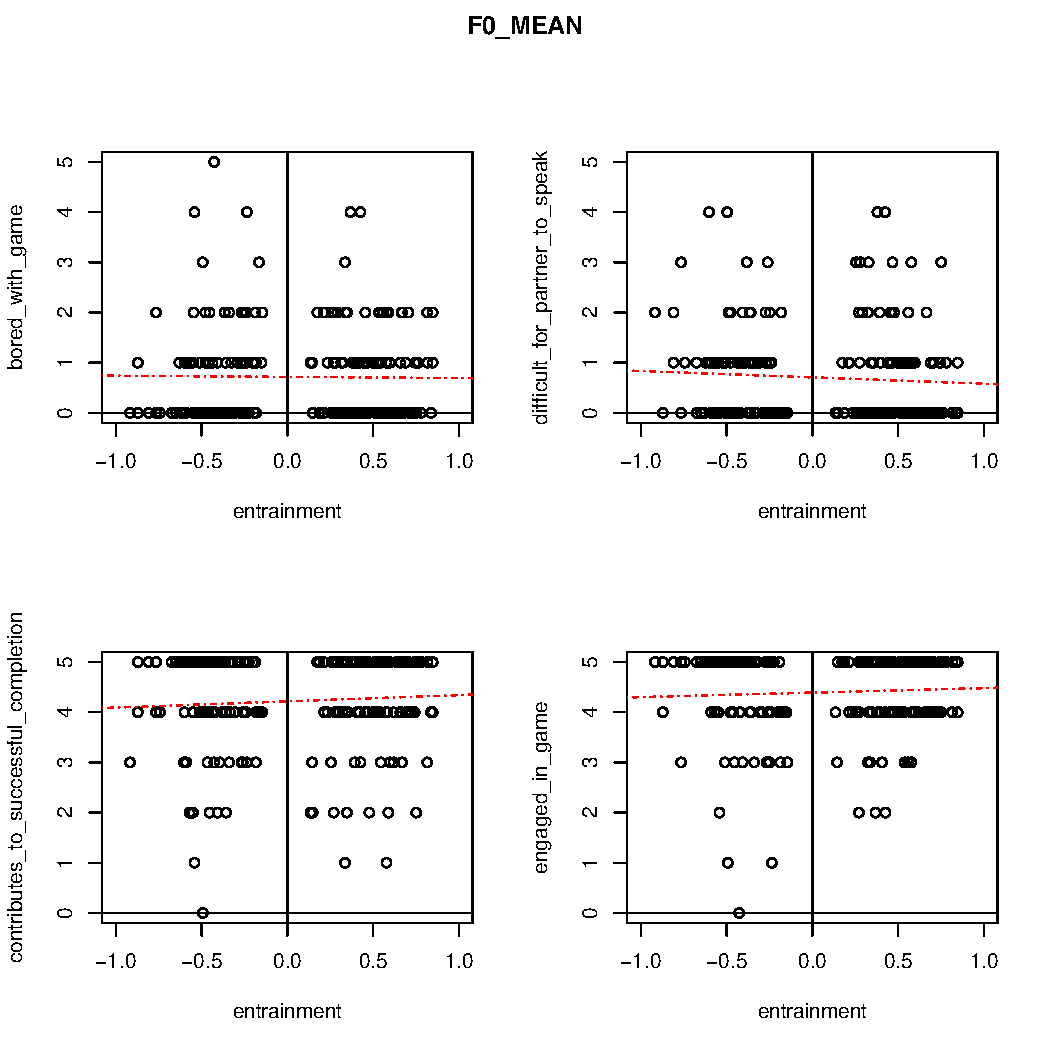
\includegraphics[width=15cm]{images/regression_F0_MEAN_1.pdf}
\caption{Gráfico de los pares entrainment-variable a/p, junto a la regresión lineal obtenida \label{regresion_clasica} para \emph{F0\_MEAN}}
\end{figure}

En el modelo clásico dio resultados con baja significancia. En \ref{regresion_clasica} puede verse el gráfico de \emph{F0\_MEAN} y 4 variables sociales y en \ref{regresion_clasica_tabla} pueden verse los valores de las estimaciones de $\estslope$ junto a sus p-valores.


% "ENG_MEAN"
% latex table generated in R 3.2.2 by xtable 1.8-0 package
% Thu Jan  7 03:01:56 2016
\begin{tabular}{rrrrr}
  \hline
 ENG\_MEAN & $\widehat{\beta_2}$ & Std. Error & t value & Pr($>$$|$t$|$) \\
  \hline
  bored\_with\_game & 10.6496 & -0 & 2.036037E-21 & 0.6587 \\
  difficult\_for\_partner\_to\_speak & 10.5625 & -1 & 3.728189E-21 & 0.5893 \\
  contributes\_to\_successful\_completion & 59.6193 & -1 & 9.639522E-133 & 0.2519 \\
  engaged\_in\_game & 73.1439 & 1 & 2.276897E-150 & 0.5851 \\
  gives\_encouragement & 47.4920 & -0 & 1.314327E-113 & 0.9659 \\
  making\_self\_clear & 52.9691 & -1 & 1.022216E-122 & 0.3253 \\
  planning\_what\_to\_say & 32.0193 & -2 & 2.465471E-82 & 0.0718 \\
  dislikes\_partner & 9.6126 & -1 & 2.462398E-18 & 0.3482 \\  \hline
\end{tabular}

% latex table generated in R 3.2.2 by xtable 1.8-0 package
% Fri Jan  8 00:50:24 2016
\begin{tabular}{rrrrr}
  \hline
 ENG\_MAX & $\widehat{\beta_2}$ & Std. Error & t value & Pr($>$$|$t$|$) \\
  \hline
bored\_with\_game & 10.4714 & 0 & 7.003232E-21 & 0.9053 \\
  difficult\_for\_partner\_to\_speak & 10.3984 & -0 & 1.160098E-20 & 0.9678 \\
  contributes\_to\_successful\_completion & 58.9660 & -0 & 8.397021E-132 & 0.6739 \\
  engaged\_in\_game & 72.6730 & 1 & 8.299021E-150 & 0.6008 \\
  gives\_encouragement & 47.3103 & -0 & 2.727411E-113 & 0.6494 \\
  making\_self\_clear & 52.2454 & 1 & 1.465061E-121 & 0.3220 \\
  planning\_what\_to\_say & 31.1729 & 0 & 2.491793E-80 & 0.7176 \\
  dislikes\_partner & 9.5924 & -1 & 2.820254E-18 & 0.3279 \\
   \hline
\end{tabular}

% latex table generated in R 3.2.2 by xtable 1.8-0 package
% Thu Jan  7 03:01:56 2016
\begin{tabular}{rrrrr}
  \hline
F0\_MEAN & $\widehat{\beta_2}$ & Std. Error & t value & Pr($>$$|$t$|$) \\
  \hline
bored\_with\_game & 10.6286 & -0 & 2.355933E-21 & 0.8572 \\
  difficult\_for\_partner\_to\_speak & 10.6764 & -1 & 1.689495E-21 & 0.3316 \\
  contributes\_to\_successful\_completion & 59.3792 & 1 & 2.130619E-132 & 0.3726 \\
  engaged\_in\_game & 73.4118 & 1 & 1.094910E-150 & 0.4425 \\
  gives\_encouragement & 47.5948 & 1 & 8.705216E-114 & 0.2774 \\
  making\_self\_clear & 52.9055 & -0 & 1.290163E-122 & 0.7471 \\
  planning\_what\_to\_say & 31.4874 & 0 & 4.441831E-81 & 0.6977 \\
  dislikes\_partner & 9.8092 & -2 & 6.530815E-19 & 0.0835 \\
   \hline
\end{tabular}

% ""
% latex table generated in R 3.2.2 by xtable 1.8-0 package
% Thu Jan  7 03:01:56 2016
\begin{tabular}{rrrrr}
  \hline
F0\_MAX & $\widehat{\beta_2}$ & Std. Error & t value & Pr($>$$|$t$|$) \\
  \hline
bored\_with\_game & 11.0806 & 2 & 1.001502E-22 & 0.0147 \\
  difficult\_for\_partner\_to\_speak & 10.6511 & 1 & 2.014306E-21 & 0.6023 \\
  contributes\_to\_successful\_completion & 60.0792 & -1 & 2.127331E-133 & 0.3297 \\
  engaged\_in\_game & 74.2016 & -1 & 1.282700E-151 & 0.5711 \\
  gives\_encouragement & 48.1664 & -1 & 8.925956E-115 & 0.2986 \\
  making\_self\_clear & 53.8649 & -2 & 3.954497E-124 & 0.0212 \\
  planning\_what\_to\_say & 31.8577 & -1 & 5.915312E-82 & 0.2950 \\
  dislikes\_partner & 9.6545 & 1 & 1.857261E-18 & 0.3340 \\
  \hline
\end{tabular}





\section{Modelo de Efectos Fijos}

\newcommand{\slopeestim}[1] { $\estslope \sim #1$ }

El modelo de efectos fijos sobre el valor absoluto del \emph{entrainment} dio valores sustancialmente más apreciables. \ENGMAX, \FOMEAN y \NOISETOHARMONICS poseen valores altamente significativos ( p-valor menor a 0.05) para la regresión con efectos fijos para al menos 2 variables sociales.

En la tabla \ref{regresion_efectos_fijos_tabla} podemos ver estos valores con las variables sociales significativas resaltadas.


\begin{figure}
\begin{figure}[p]
\centering
\adjustbox{max width=\textwidth}{
\begin{tabular}{rrrrr}
  \hline
\ENGMAX & $\estslope$ & Std. Error & t value & Significance \\ 
  \hline
contributes\_to\_successful\_completion & 0.0720 & 0.4258 & 1.689631E-01 & 0.8660 \\ 
  \stronghl making\_self\_clear & 1.6914 & 0.3820 & 4.427376E+00 & 0.0000 \\ 
  engaged\_in\_game & 0.3456 & 0.2528 & 1.367266E+00 & 0.1732 \\ 
  planning\_what\_to\_say & 0.5655 & 0.5208 & 1.085851E+00 & 0.2790 \\ 
  gives\_encouragement & 0.4739 & 0.3744 & 1.265523E+00 & 0.2073 \\ 
  \stronghl difficult\_for\_partner\_to\_speak & -0.6925 & 0.2863 & -2.418510E+00 & 0.0166 \\ 
  bored\_with\_game & 0.2110 & 0.2543 & 8.298495E-01 & 0.4077 \\ 
  dislikes\_partner & -0.4254 & 0.3438 & -1.237312E+00 & 0.2175 \\ 

  \hline
\ENGMEAN & $\estslope$ & Std. Error & t value & Significance \\ 
  \hline
  \softhl contributes\_to\_successful\_completion & 0.6552 & 0.3610 & 1.814712E+00 & 0.0712 \\ 
  making\_self\_clear & 0.9470 & 0.6080 & 1.557502E+00 & 0.1211 \\ 
  \softhl engaged\_in\_game & 0.7091 & 0.3847 & 1.843187E+00 & 0.0669 \\ 
  planning\_what\_to\_say & 0.3636 & 0.5756 & 6.316937E-01 & 0.5284 \\ 
  gives\_encouragement & 0.4051 & 0.3482 & 1.163506E+00 & 0.2461 \\ 
  \hl difficult\_for\_partner\_to\_speak & 0.5287 & 0.2515 & 2.101960E+00 & 0.0369 \\ 
  bored\_with\_game & -0.0036 & 0.4106 & -8.663987E-03 & 0.9931 \\ 
  dislikes\_partner & 0.5307 & 0.3889 & 1.364514E+00 & 0.1741 \\ 

  \hline
\FOMEAN & $\estslope$ & Std. Error & t value & Significance \\ 
  \hline
  \stronghl contributes\_to\_successful\_completion & 0.9752 & 0.3058 & 3.188448E+00 & 0.0017 \\ 
  \softhl making\_self\_clear & 0.6998 & 0.3907 & 1.791239E+00 & 0.0749 \\ 
  \stronghl engaged\_in\_game & 0.8538 & 0.2773 & 3.078945E+00 & 0.0024 \\ 
  planning\_what\_to\_say & 0.6430 & 0.5363 & 1.198966E+00 & 0.2321 \\ 
  gives\_encouragement & 0.0006 & 0.3885 & 1.577445E-03 & 0.9987 \\ 
  difficult\_for\_partner\_to\_speak & -0.5323 & 0.3835 & -1.388190E+00 & 0.1667 \\ 
  \stronghl bored\_with\_game & -0.7663 & 0.2582 & -2.968508E+00 & 0.0034 \\ 
  dislikes\_partner & 0.0688 & 0.3808 & 1.806265E-01 & 0.8569 \\ 

\FOMAX & $\estslope$ & Std. Error & t value & Significance \\ 
  \hline
  \softhl contributes\_to\_successful\_completion & 0.7628 & 0.4381 & 1.741129E+00 & 0.0833 \\ 
  making\_self\_clear & 0.6718 & 0.4129 & 1.626984E+00 & 0.1054 \\ 
  engaged\_in\_game & 0.5308 & 0.3776 & 1.405582E+00 & 0.1615 \\ 
  planning\_what\_to\_say & 0.0489 & 0.4210 & 1.161167E-01 & 0.9077 \\ 
  gives\_encouragement & 0.4724 & 0.5464 & 8.647145E-01 & 0.3883 \\ 
  difficult\_for\_partner\_to\_speak & -0.3208 & 0.2821 & -1.136927E+00 & 0.2570 \\ 
  bored\_with\_game & -0.2584 & 0.3764 & -6.865032E-01 & 0.4933 \\ 
  dislikes\_partner & 0.1249 & 0.3884 & 3.216226E-01 & 0.7481 \\ 
\end{tabular}}

\caption{Tablas con los resultados de la regresión de efectos fijos sobre el va,or absoluto de \entrainment para \ENGMAX, \ENGMEAN, \FOMEAN y \FOMAX. En la segunda columna se cita el valor de $\estslope$, la desviación estándar calculada, el t-valor obtenido y la significancia. Las columnas resaltadas corresponden a aquellas significantes, con diferentes matices de gris según $p < 0.10$, $p < 0.5$, o $p < 0.01$}
\label{fig:efectos_fijos_tabla1}

\end{figure}




\begin{figure}[pt!]
\centering
\adjustbox{max width=\textwidth}{
\begin{tabular}{rrrrr}
  \hline
  \hline
\NOISETOHARMONICS & $\estslope$ & Std. Error & t value & Significance \\ 
  \hline
  \hl contributes\_to\_successful\_completion & 0.7271 & 0.3439 & 2.114275E+00 & 0.0358 \\ 
  \stronghl making\_self\_clear & 1.3576 & 0.3613 & 3.758007E+00 & 0.0002 \\ 
  engaged\_in\_game & 0.1270 & 0.3431 & 3.702043E-01 & 0.7117 \\ 
  planning\_what\_to\_say & -0.1625 & 0.4264 & -3.811856E-01 & 0.7035 \\ 
  gives\_encouragement & 0.7665 & 0.4860 & 1.577201E+00 & 0.1165 \\ 
  difficult\_for\_partner\_to\_speak & -0.1683 & 0.3400 & -4.951813E-01 & 0.6211 \\ 
  \softhl bored\_with\_game & 0.5527 & 0.3084 & 1.792251E+00 & 0.0747 \\ 
  dislikes\_partner & 0.3457 & 0.3279 & 1.054410E+00 & 0.2931 \\ 
   \hline

  \hline
\PHONAVG & $\estslope$ & Std. Error & t value & Significance \\ 
  \hline
contributes\_to\_successful\_completion & 0.5557 & 0.3577 & 1.553747E+00 & 0.1220 \\ 
  making\_self\_clear & 0.7598 & 0.5085 & 1.494093E+00 & 0.1369 \\ 
  engaged\_in\_game & 0.2440 & 0.2586 & 9.438356E-01 & 0.3465 \\ 
  planning\_what\_to\_say & 0.3614 & 0.5174 & 6.984626E-01 & 0.4858 \\ 
  gives\_encouragement & 0.0604 & 0.3829 & 1.576928E-01 & 0.8749 \\ 
  \softhl difficult\_for\_partner\_to\_speak & -0.6264 & 0.3374 & -1.856257E+00 & 0.0650 \\ 
  bored\_with\_game & -0.0158 & 0.3204 & -4.921947E-02 & 0.9608 \\ 
  dislikes\_partner & 0.0975 & 0.3137 & 3.108070E-01 & 0.7563 \\ 
   \hline

\SYLAVG & $\estslope$ & Std. Error & t value & Significance \\ 
  \hline
  contributes\_to\_successful\_completion & 0.2451 & 0.3663 & 6.692398E-01 & 0.5042 \\ 
  \softhl making\_self\_clear & 0.7934 & 0.4094 & 1.937743E+00 & 0.0542 \\ 
  engaged\_in\_game & 0.4956 & 0.3642 & 1.360687E+00 & 0.1753 \\ 
  planning\_what\_to\_say & 0.4429 & 0.5189 & 8.535430E-01 & 0.3945 \\ 
  gives\_encouragement & 0.2363 & 0.4192 & 5.637211E-01 & 0.5736 \\ 
  difficult\_for\_partner\_to\_speak & 0.1856 & 0.3481 & 5.332959E-01 & 0.5945 \\ 
  bored\_with\_game & -0.2909 & 0.3606 & -8.067536E-01 & 0.4208 \\ 
  dislikes\_partner & 0.1768 & 0.3452 & 5.120454E-01 & 0.6092 \\ 
   \hline

  \hline
\LOCALJITTER & $\estslope$ & Std. Error & t value & Significance \\ 
  \hline
contributes\_to\_successful\_completion & 0.5770 & 0.3759 & 1.534821E+00 & 0.1265 \\ 
  making\_self\_clear & 0.5057 & 0.4881 & 1.036143E+00 & 0.3015 \\ 
  \hl engaged\_in\_game & 0.4972 & 0.2515 & 1.977130E+00 & 0.0495 \\ 
  planning\_what\_to\_say & -0.0417 & 0.4628 & -9.000210E-02 & 0.9284 \\ 
  gives\_encouragement & -0.0160 & 0.3502 & -4.554031E-02 & 0.9637 \\ 
  difficult\_for\_partner\_to\_speak & -0.2788 & 0.3126 & -8.917922E-01 & 0.3737 \\ 
  bored\_with\_game & 0.1233 & 0.3155 & 3.906725E-01 & 0.6965 \\ 
  dislikes\_partner & -0.1171 & 0.2788 & -4.198582E-01 & 0.6751 \\ 
  \hline
\LOCALSHIMMER & $\estslope$ & Std. Error & t value & Significance \\ 
  \hline
contributes\_to\_successful\_completion & 0.3745 & 0.2754 & 1.359709E+00 & 0.1756 \\ 
  making\_self\_clear & -0.0097 & 0.3821 & -2.544762E-02 & 0.9797 \\ 
  engaged\_in\_game & 0.2434 & 0.2881 & 8.449092E-01 & 0.3993 \\ 
  planning\_what\_to\_say & -0.6040 & 0.4735 & -1.275476E+00 & 0.2037 \\ 
  \softhl gives\_encouragement & 0.3638 & 0.2057 & 1.768094E+00 & 0.0787 \\ 
  difficult\_for\_partner\_to\_speak & 0.2707 & 0.2720 & 9.952034E-01 & 0.3209 \\ 
  bored\_with\_game & -0.3635 & 0.2772 & -1.311203E+00 & 0.1914 \\ 
  dislikes\_partner & -0.1895 & 0.2667 & -7.105564E-01 & 0.4783 \\ 
\end{tabular}}

\caption{Tablas con los resultados de la regresión de efectos fijos para \NOISETOHARMONICS, \SYLAVG, \PHONAVG, \LOCALSHIMMER y \LOCALJITTER. En la segunda columna se cita el valor de $\estslope$, la desviación estándar calculada, el t-valor obtenido y la significancia. Las columnas resaltadas corresponden a aquellas significantes, con diferentes matices de gris según $p < 0.10$, $p < 0.5$, o $p < 0.01$}

\label{fig:efectos_fijos_tabla2}
\end{figure}

\caption{Tablas con los resultados de la regresión de efectos fijos para \ENGMAX, \FOMEAN y \NOISETOHARMONICS. En la segunda columna se cita el valor de $\estslope$, la desviación estándar calculada, el t-valor obtenido y la significancia. Las columnas resaltadas corresponden a aquellas significantes}\label{regresion_efectos_fijos_tabla}
\end{figure}
